\documentclass[tikz,border=5pt]{standalone}
\usepackage{tikz}
\usetikzlibrary{arrows.meta,positioning,calc}
\definecolor{nebula}{HTML}{6366F1}
\definecolor{spark}{HTML}{14B8A6}
\definecolor{ink}{HTML}{334155}
\begin{document}
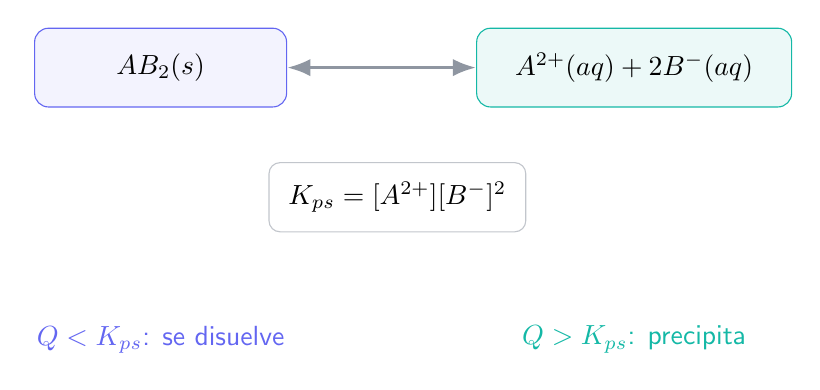
\begin{tikzpicture}[font=\sffamily,>=Latex,node distance=1.6cm]
  \node[draw=nebula,rounded corners=5pt,fill=nebula!8,minimum width=3.2cm,minimum height=1cm] (solid)
    {$AB_2(s)$};
  \node[draw=spark,rounded corners=5pt,fill=spark!8,minimum width=4cm,minimum height=1cm,right=2.4cm of solid] (ions)
    {$A^{2+}(aq)+2B^-(aq)$};
  \draw[<->,very thick,ink!55] (solid)--(ions);
  \node[draw=ink!30,rounded corners=4pt,fill=white,inner sep=7pt,below=1.2cm of $(solid)!0.5!(ions)$]
    {$K_{ps}=[A^{2+}][B^-]^2$};
  \node[text=nebula,below=2.65cm of solid] {$Q<K_{ps}$: se disuelve};
  \node[text=spark,below=2.65cm of ions] {$Q>K_{ps}$: precipita};
\end{tikzpicture}
\end{document}
